\documentclass[a4paper,10pt]{article}

\usepackage[utf8]{inputenc}
\usepackage{amsmath}
\usepackage{csquotes}% Recommended
\usepackage{amssymb}

\usepackage{mathtools}
\DeclarePairedDelimiter{\ceil}{\lceil}{\rceil}
\DeclarePairedDelimiter{\floor}{\lfloor}{\rfloor}

% pseudo code packages
\usepackage{algorithm}
\usepackage[noend]{algpseudocode}
\algnewcommand\algorithmicto{\textbf{to}}
\algrenewtext{For}[3]{\algorithmicfor\ $#1 \gets #2$ \algorithmicto\ $#3$ \algorithmicdo}
\makeatletter
\def\BState{\State\hskip-\ALG@thistlm}
\makeatother

\usepackage[ddmmyyyy]{datetime}
\renewcommand{\dateseparator}{/}

% Harward Referencing
\usepackage[UKenglish]{babel}
\usepackage[style=authoryear-ibid,backend=biber]{biblatex}

% Citation file
\addbibresource{citation.bib}

% Verbatim environment
\usepackage{listings}
\lstdefinestyle{code}{
  basicstyle=\small\ttfamily,
  columns=flexible,
  breaklines=true
}
\lstset{style=code}

\usepackage{pgfplots}

% Title Page
\title{LaTeX - The Document Preparation System}
\author{Frederick Zhang}
\date{\today}

\begin{document}
\maketitle

\begin{abstract}
A brief introduction to LaTeX.
\newline\textbf{Keyword}: LaTeX
\end{abstract}

\section{Introduction}
LaTeX was first developed in the early 1980s by Leslie Lamport, and it was based on Donald E. Knuth's TeX typesetting language. \autocite{8732314920150101}
\newline Latex is a stable dispersion (emulsion) of polymer microparticles in an aqueous medium. It is found in nature, but synthetic latexes can be made by polymerizing a monomer such as styrene that has been emulsified with surfactants. \autocite{LaTeXWiki}

\section{Basic}
\begin{enumerate}
  \item Enum 1
  \newline Hello World
  
  \item Enum 2
  \newline \textcolor{red}{I can eat glass, it doesn't hurt me.}
\end{enumerate}
\begin{itemize}
  \item [Item I] The quick brown fox jumps over the lazy dog.
  \item [Item II] Foo Bar
\end{itemize}

\section{Table}
\begin{tabular}{l | r | r}
  Col 1 & Col 2 & Col 3 \\ \hline
  Hello & 128 & 256 \\
  World & 512 & 1024
\end{tabular}

\section{Formula}
\begin{enumerate}
  \item Sample 1
  $$ s_N=\sqrt{\frac{1}{N} \sum_{i=1}^{N} (x_i - \overline{x})^2} $$
  
  \item Sample 2
  $$ f(x;\mu,\sigma) = \frac{1}{\sigma\sqrt{2\pi}}exp(-\frac{(x-\mu)^2}{2\sigma^2}) $$
  
  \item Sample 3
  $$ \hat{f}(\xi)=\int_{-\infty}^{\infty} f(x) e^{-2\pi ix\xi} $$
\end{enumerate}

\section{Chart}
There are generally two suggested approaches to generate charts in LaTeX - \textsf{pgfplots} and \textsf{gnuplot}.
\newline \textsf{pgfplots} is a package for LaTeX and it's easier to use.
\begin{enumerate}
  \item Sample 1
  \newline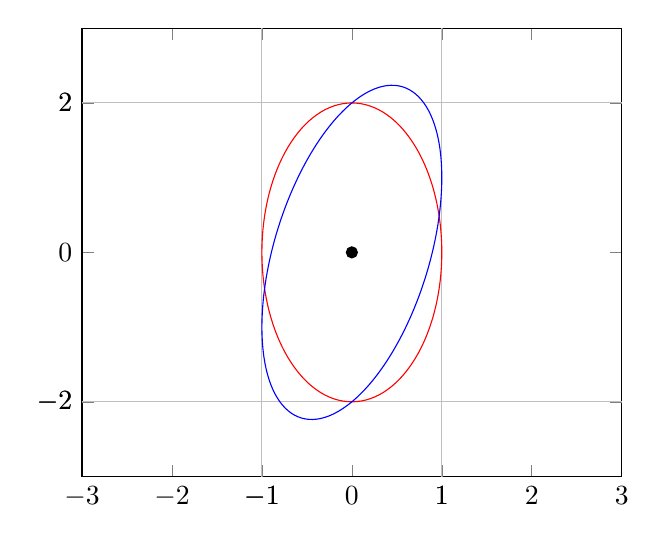
\begin{tikzpicture}
  \begin{axis}[
	  xmin=-3,   xmax=3,
	  ymin=-3,   ymax=3,
	  extra x ticks={-1,1},
	  extra y ticks={-2,2},
	  extra tick style={grid=major},
  ]
	  \draw[red] \pgfextra{
	    \pgfpathellipse{\pgfplotspointaxisxy{0}{0}}
		  {\pgfplotspointaxisdirectionxy{1}{0}}
		  {\pgfplotspointaxisdirectionxy{0}{2}}
	    % see also the documentation of 
	    % 'axis direction cs' which
	    % allows a simpler way to draw this ellipse
	  };
	  \draw[blue] \pgfextra{
	    \pgfpathellipse{\pgfplotspointaxisxy{0}{0}}
		  {\pgfplotspointaxisdirectionxy{1}{1}}
		  {\pgfplotspointaxisdirectionxy{0}{2}}
	  };
	  \addplot [only marks,mark=*] coordinates { (0,0) };
  \end{axis}
  \end{tikzpicture}
  
  \item Sample 2
  \newline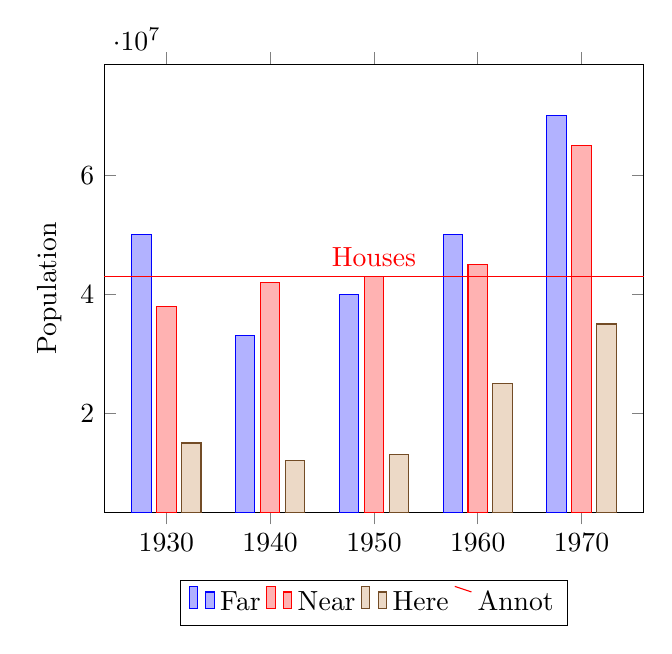
\begin{tikzpicture}
  \begin{axis}[
	  x tick label style={
		  /pgf/number format/1000 sep=},
	  ylabel=Population,
	  enlargelimits=0.15,
	  legend style={at={(0.5,-0.15)},
		  anchor=north,legend columns=-1},
	  ybar,
	  bar width=7pt,
  ]
  \addplot 
	  coordinates {(1930,50e6) (1940,33e6)
		  (1950,40e6) (1960,50e6) (1970,70e6)};

  \addplot 
	  coordinates {(1930,38e6) (1940,42e6) 
		  (1950,43e6) (1960,45e6) (1970,65e6)};

  \addplot 
	  coordinates {(1930,15e6) (1940,12e6) 
		  (1950,13e6) (1960,25e6) (1970,35e6)};

  \addplot[red,sharp plot,update limits=false] 
	  coordinates {(1910,4.3e7) (1990,4.3e7)} 
	  node[above] at (axis cs:1950,4.3e7) {Houses};

  \legend{Far,Near,Here,Annot}
  \end{axis}
  \end{tikzpicture}
  
  \newpage\item Sample 3
  \newline
  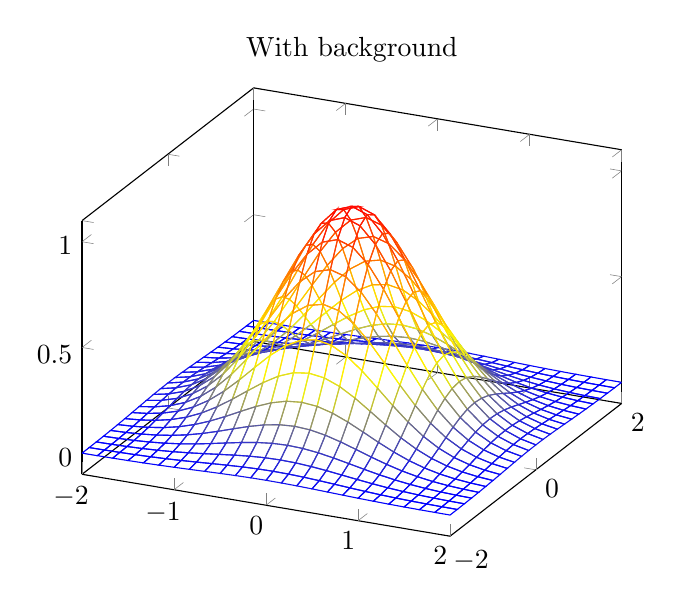
\begin{tikzpicture}
	  \begin{axis}[title=With background]
	  \addplot3[mesh,domain=-2:2] {exp(-x^2-y^2)};	
	  \end{axis}
  \end{tikzpicture}
  \newline
  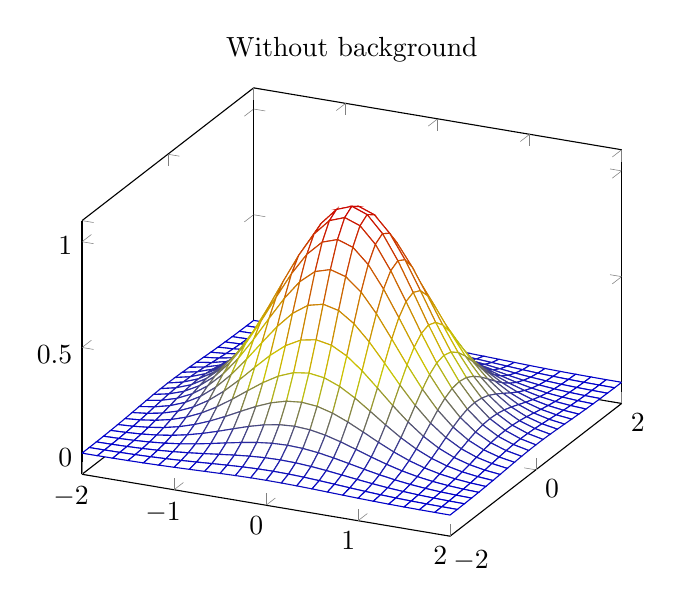
\begin{tikzpicture}
	  \begin{axis}[title=Without background]
	  \addplot3[surf,fill=white,domain=-2:2] {exp(-x^2-y^2)};	
	  \end{axis}
  \end{tikzpicture}
\end{enumerate}

\section{Referencing}
The \textit{Harward Referencing} is preferred in Australia.
\newline We use \textsf{biber} and \textsf{biblatex} to manage the citations.
\newline Biber is a bibliography information processing program and works in conjunction with the LaTeX package biblatex and offers full Unicode support. \autocite{BiberWiki}

\section{Pseudo-code}
\textit{algorithmicx} is suggested to handle pseudo-codes. To make use of it, we need two packages - \textsf{algorithm} and \textsf{algpseudocode}.
\begin{enumerate}
  \item Sample 1
  \newline\begin{algorithm}
    \caption{Sample 1}
    \begin{algorithmic}
      \Function{HelloWorld}{n}
	\For{i}{0}{n-1} \Comment print n ``hello''s
	  \State \Call{PrintLine}{hello}
	\EndFor
      \EndFunction
    \end{algorithmic}
  \end{algorithm}
  
  \item Sample 2
  \begin{algorithm}
    \caption{Sample 2}
    \begin{algorithmic}[2]
      \Function{Triangulable}{$P[0..n-1]$}
      \Comment elements of P are pairs $<x, y>$
        \If{$n < 3$}
          \State \Return $false$
        \EndIf
        \For{i}{0}{n-2}
          \State $array[0..n-i-1] \gets [null..null]$
          \For{j}{i+1}{n-1}
            \State $x1, y1 \gets P[i]$
            \State $x2, y2 \gets P[j]$
            \If{$x1 \neq x2$}
              \State $slope \gets (y2-y1)/(x2-x1)$
            \Else
              \State $slope \gets null$
            \EndIf
            \State $array[j-i-1] \gets slope$
          \EndFor
          \State \Call{HeapSort}{$array$}
          \Comment introduced in Week 7 lecture
          \For{j}{1}{n-i-2}
            \If{$array[j] = array[j+1]$}
              \State \Return $false$
            \EndIf
          \EndFor
        \EndFor
        \State \Return $true$
      \EndFunction
    \end{algorithmic}
  \end{algorithm}
\end{enumerate}

\section{Suggested Online Resources}
https://en.wikibooks.org/wiki/LaTeX
\newline https://tex.stackexchange.com/
\newline https://www.ctan.org/
\newline http://pgfplots.sourceforge.net/

\newpage
\printbibliography

\end{document}
